
% \subsection{Secciones del circuito}

\begin{figure}[H] %htb
\begin{center}
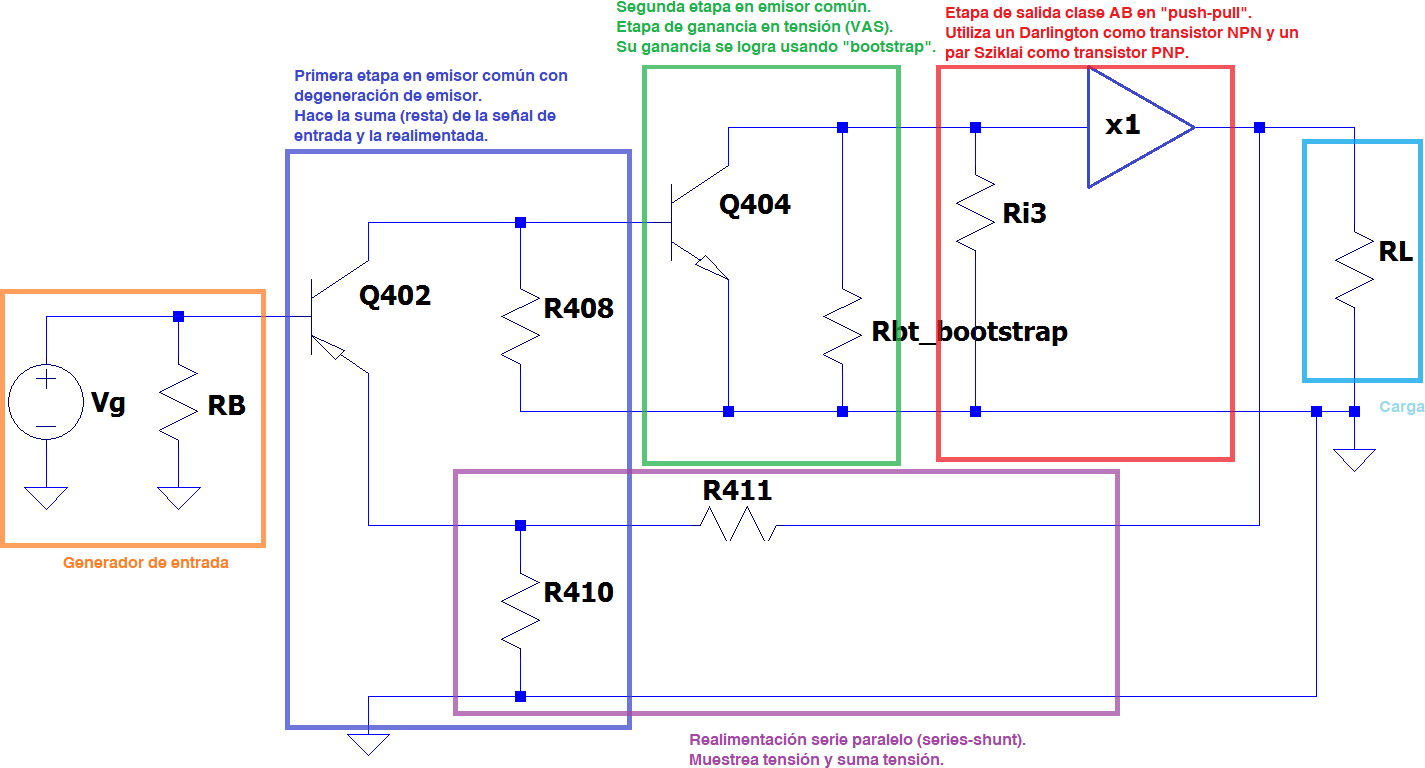
\includegraphics[width=0.9 \textwidth, angle=0]{./img/desarrollo/0_etapas.png}
\caption{\label{fig:fig_complete_circuit_stages}\footnotesize{Circuito esquematizado con las etapas indicadas.}}
\end{center}
\end{figure}



En la figura~\figref{fig:fig_complete_circuit_stages} se muestra el circuito de señal simplificado del amplificador, en donde se detallan las etapas que lo conforman, se trata de las tres típicas etapas de un amplificador de potencia, una primera etapa en emisor común con degeneración de emisor, donde se realiza la suma (resta) de la señal de entrada y la realimentada, esta etapa, como se verá mas adelante en la sección~\sectref{stages_gain}, tiene muy poca ganancia de tensión, una segunda etapa (\textbf{VAS}), en emisor común, que gana casi toda la ganancia en tensión en el amplificador, esta etapa contiene también el circuito multiplicador de $V_{BE}$ que polariza la siguiente etapa, no se muestra en este esquema simplificado. Finalmente tenemos una etapa de salida \textbf{clase A-B}, un \textbf{push-pull} implementado con transistores compuestos, donde el transistor \textbf{NPN} está conformado por un \textbf{Darlington} y el transistor \textbf{PNP} está conformado por un par \textbf{Sziklai}.\\

Los pares compuestos de la etapa de salida tienen además unas resistencias de degeneración de emisor para mejorar la estabilidad térmica, además de que el transistor del \textbf{Darlington} está térmicamente acoplado al transistor del multiplicador de $V_{BE}$, de manera de compensarlo térmicamente. Los transistores de salida de ambos pares van montados sobre disipadores, como el cálculo en la sección~\sectref{thermal_calculation}, muestra que es necesario.\\

La realimentación \textbf{serie-paralelo} (series-shunt) estabiliza la ganancia de tensión, ya que como se demuestra en la sección~\sectref{loop_gain}, la ganancia de lazo, es mucho mayor a $1$.\\

El amplificador no amplifica desde continua, ya que además de estar acoplado con un capacitor el generador de entrada (el punto de entrada no está a tensión nula), se tienen otros capacitores que desacoplan para la señal otras partes del circuito, con lo que se espera tener una frecuencia de corte inferior, cosa que es aceptable para un amplificador de audio, como lo es en este caso.




\normalfont

